\section{Black box modeling approach}

% Difference with bottom-up, not the same application, not the same goal
The black-box modeling method relies on the same core principles than the bottom-up modeling approach.
It studies the relationship and transfert function between the input and the output of a silicon function.
Unlike the bottom-up method though, the model is only built \textbf{for external input and output pins}.
It is not meant to be chained with other models, using a special chaining method.
Instead, it targets electrical, board-level circuit simulations.
Basically, the black box model is intented to act as a drop-in replacement for the complete \gls{ic} circuit, for board-level simulations.

% What is the motivation
%TODO: Reference for SEED
The purpose is also different from the bottom-up approach.
The goal is not to detect issues at silicon-level early before manufacturing, but to let customers using the \gls{ic} in a \gls{pcb} to detect issues with the board that could result in silicon-functions failure.
The \gls{seed} methodology recommends to design systems in a smart fashion for making them robust during operation, which requires a collaboration between board-level and silicon-level protective measures.
Ultimately, the goal is to provide a black box model that is \textbf{fast to simulate} and can be \textbf{distributed without disclosing sensitive intellectual property}.

% introduction, failure relation between input and output
The main benefit of this model is to abstract the internal silicon complexity.
The model focuses on describing the failure of an output when an input is stressed.
At board-level, failure criteria can be more easily set from the chip specification.
After setting the failure criteria, the approach is to inject rectangular pulses on an input pin, and record when an output is in fault.

% access to the signals
Since the characterized nets are external pins, they are physically accessible.
Thus, the black box models can be derived from actual measurements.

\subsection{Failure model}

% How is the characterization conducted
Once again, a variable width/variable amplitude rectangular pulses are applied on an input pin.
The output pin is then observed to detect for which input parameters it is going out of specification.

% What is characterized
This characterization is performed on the testchip, on the complete regulation function.
The characterization pulses are injected on the $V_{batt}$ input.
The output pin is $V_{2p5}$, the regulated supply.
It is supposed to deliver a 2.5V regulated supply.
The failure criteria is set at a voltage below 2.1V.
It corresponds to a level below which digital cells powered by this supply will have noise margins too small for proper operation.

% Fig X shows the waveform of the VBAT injected current when stressed with a TLP (square) impulse.
% The TLP waveform before the capacitor is shown for reference.
%TODO: WAVEFORM CURRENT VBAT AND TLP BEFORE INJECTION CAPACITOR ?

% Detail the characterization
The characterization table is plotted in Fig. \ref{fig:cz-black-box}.
X-axis is the pulse width, and y-axis is the minimal stress amplitude that caused a failure on the output.

\begin{figure}[!h]
  \centering
  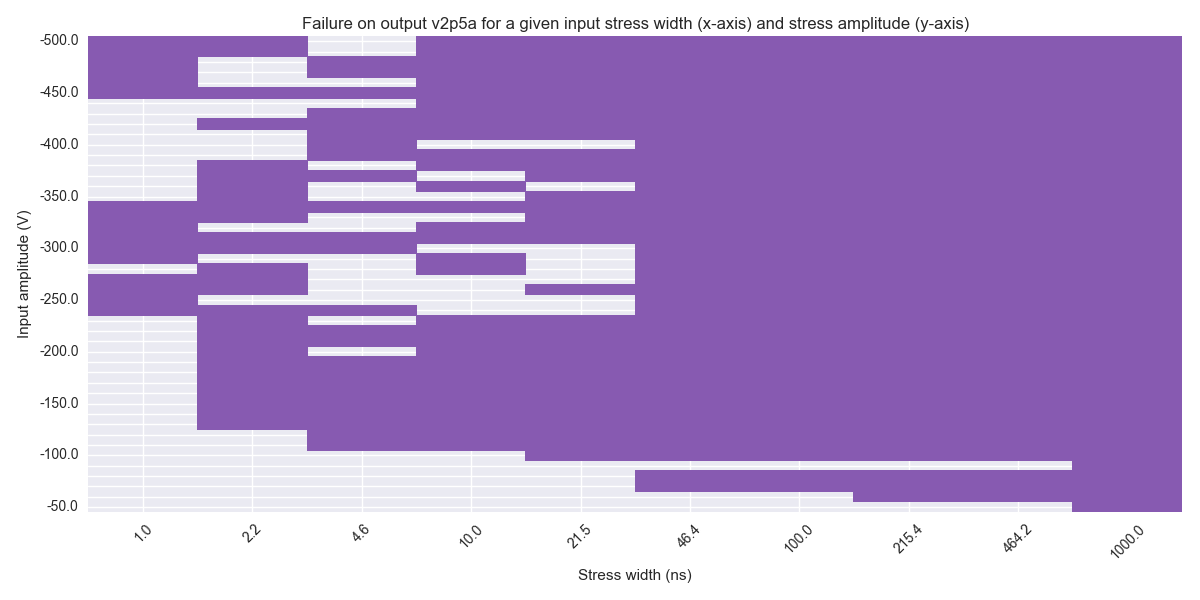
\includegraphics[width=\textwidth]{src/4/figures/black_box_regulator.png}
  \caption{Black-box characterization of the regulation function}
  \label{fig:cz-black-box}
\end{figure}

% What to do with that
%TODO: We that below this value the function is in fail, etc
However, the motivation for this model is to replace the transistor-level schematic inside a SPICE simulation at board-level.
Given a pulse width and an amplitude on $V_{batt}$, the model can estimate the disturbance amplitude and width on $V_{2p5}$.
However, the model itself is not an electrical model, only a failure model.
It cannot determinate, given for instance an input voltage, how much current is flowing into it.
This is also true for the output.
Thus, this method calls for an electrical model of \gls{io}.
The next section details how to solve this issue.

\subsection{Electrical modeling of inputs and outputs}

Need to model a silicon function, between an input external pin and output external pin.
Need an electrical model.
Hypothesis is functions IO can be modeled by their TLP characteristic (quasi-static I(V) response).

In powered or unpowered conditions ?
Unpowered conditions is the simplest, because can be done without external components.
Powered conditions is more challenging, because what to do with external devices ?

First, compare TLP curves on our regulation function, in powered and unpowered conditions.
Not interested in nominal functionnality here, just impedances.
Function does not have to be functionnal, just biased correctly.
Do not connect external devices.

\begin{figure}[!h]
  \centering
  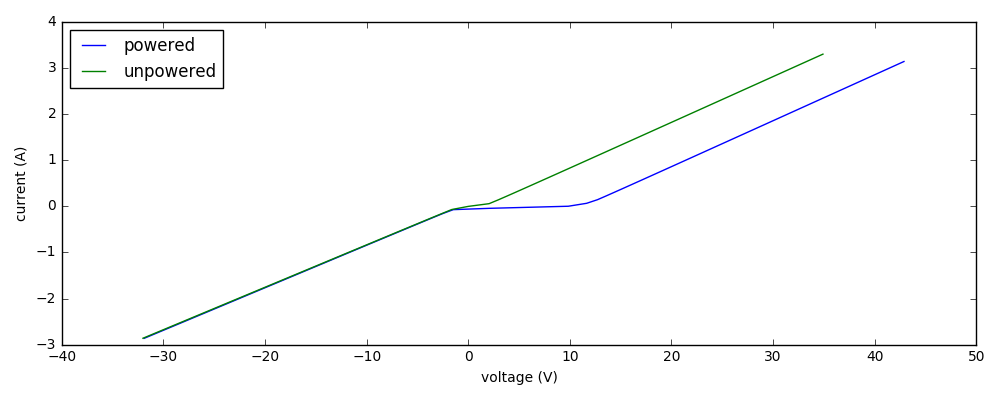
\includegraphics[width=\textwidth]{src/4/figures/tlp_input_characterization.png}
  \caption{TLP characterization of function input in powered and unpowered conditions}
  \label{fig:tlp-input-cz}
\end{figure}

\begin{figure}[!h]
  \centering
  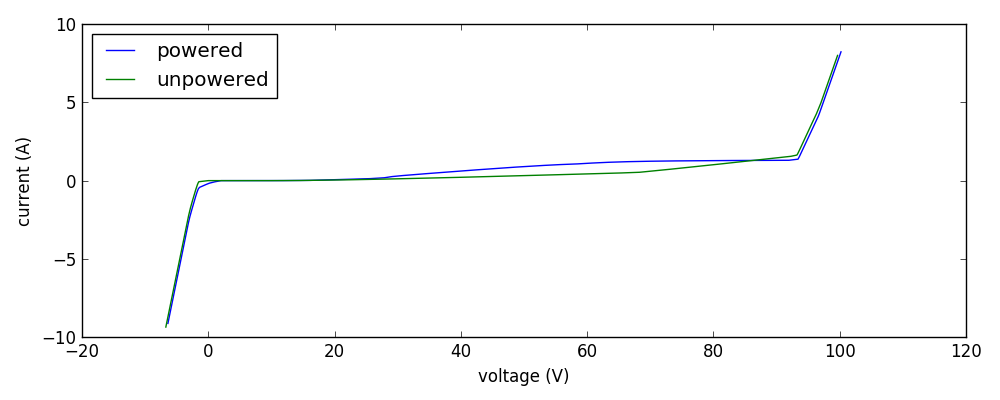
\includegraphics[width=\textwidth]{src/4/figures/tlp_output_characterization.png}
  \caption{TLP characterization of function output in powered and unpowered conditions}
  \label{fig:tlp-output-cz}
\end{figure}

For both input and output, large differences between powered and unpowered modes.
Different amount of current are absorbed by the device in each conditions.
To be as close as possible as the normal testing conditions, characterization should be done in powered conditions.

% Explain the PWL model
Second step to build an electrical model of the function
Create a piecewise linear model of the input, and of the output.
For this purpose, a generic four-points piecewise linear model was written in Verilog-A (TODO: Ref).
Configured with 4 four (V\textsubscript{i},I\textsubscript{i}) points.

\lstset{style=veriloga-style}
\lstinputlisting[caption=Piecewise-linear 4 points model, float, linerange={1-21}, firstnumber=1]{src/4/snippets/pwl_4pts.va}

% Comment the model
Convergence can be difficult to achieve
Must ensure that the PWL is continuous
Also, curves are extracted for a wide range of voltages.
However, it is an integrated function and not an ESD protection.
Thus, any part of the curve beyond the upstream ESD protection triggering-voltage is useless, since voltage will never reach this area.
Also, any part of the curve beyond the Safe-Operating Area (TODO: gloss) of the function is also useless.
Device will be destroyed beyond this limit, in which case we are not interested in functional failures anymore.
Finally, it was observed that rather than trying to fit properly the entire curve with the PWL, it is very important to fit the curve near the nominal voltage.
In our case, between -10V and 40V.


% Validate the model with TLP
Compare full-transistor simulation (nominal + esd) with the input model.
After issues described previously were solved, good agreement is achieved between model and complete circuit, at -10V, 20V and 40V TLP amplitude.
%TODO: Comment waveforms

\begin{figure}[!h]
  \centering
  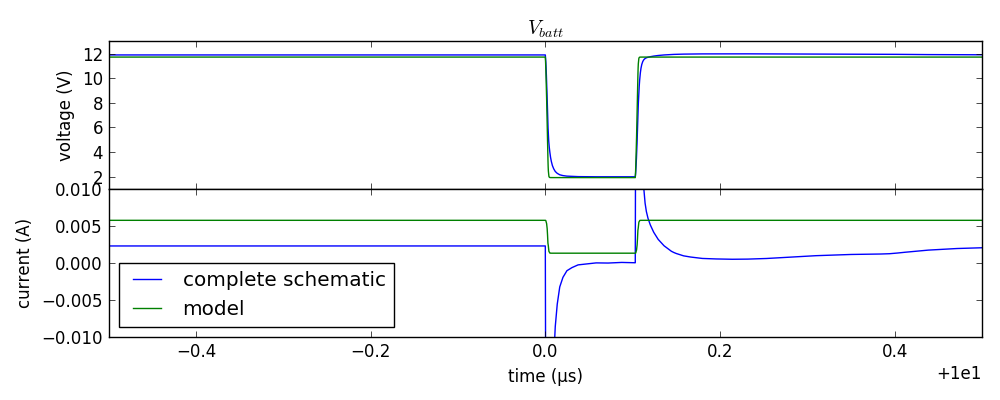
\includegraphics[width=\textwidth]{src/4/figures/comparison_model_total_m10V.png}
  \caption{Comparison of complete schematic and model simulations - -10V TLP}
  \label{fig:compare-model-simu-m10}
\end{figure}

\begin{figure}[!h]
  \centering
  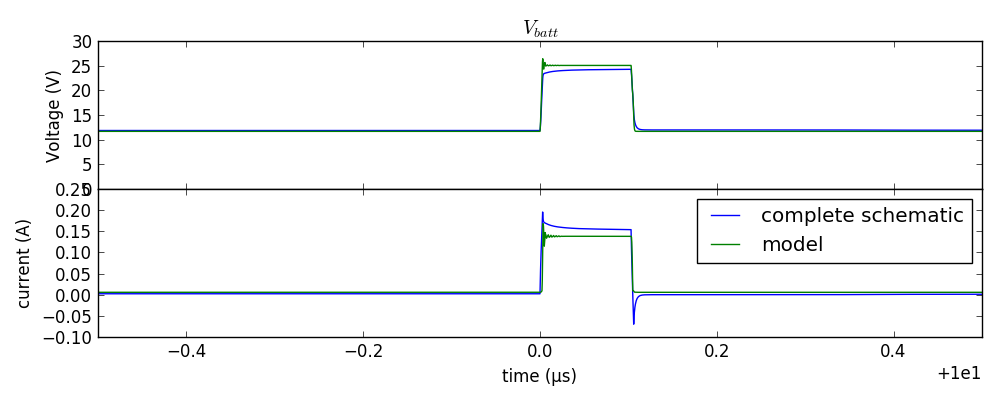
\includegraphics[width=\textwidth]{src/4/figures/comparison_model_total_20V.png}
  \caption{Comparison of complete schematic and model simulations - 20V TLP}
  \label{fig:compare-model-simu-20}
\end{figure}

\begin{figure}[!h]
  \centering
  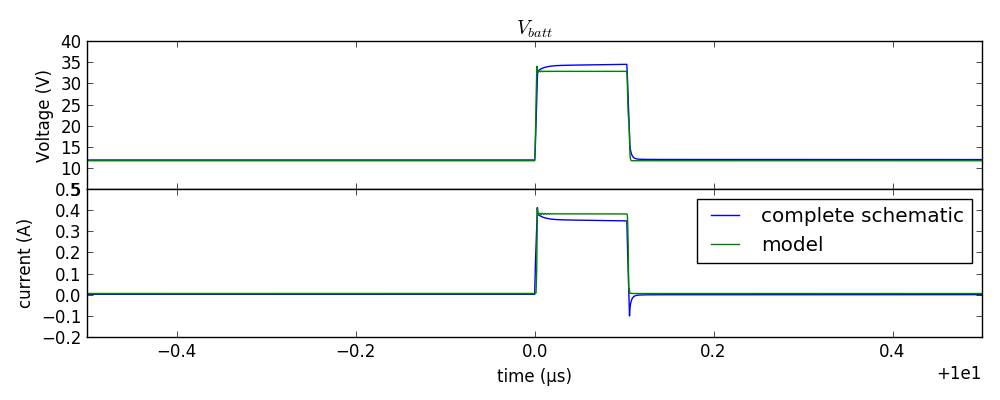
\includegraphics[width=\textwidth]{src/4/figures/comparison_model_total_40V.png}
  \caption{Comparison of complete schematic and model simulations - 40V TLP}
  \label{fig:compare-model-simu-40}
\end{figure}

%TODO: Move as opening ?
Also, need to validate with a varying waveform

\subsection{Combining failure and electrical models}

% What is the complete model
The complete function model combines the input piecewise-linear model, the failure model, the output piecewise-linear model, and an output DC source (for settling nominal value).

Fig. \ref{fig:complete-black-box-model}
The failure model act as a voltage-controlled voltage source, controlled by the input, and acting on the output.
Given an disturbance amplitude and width and width on the input, it configures and generates a rectangular pulse on the output.

\begin{figure}[!h]
  \centering
  \includegraphics[width=0.3\textwidth]{src/4/figures/complete_black_box_model.pdf}
  \caption{Architecture of the complete black-box model}
  \label{fig:complete-black-box-model}
\end{figure}

% how is this model
To test the entire concept, two simulations are run.
The first one is the classic, transistor-level simulation of the function exposed to a (XX V, XXX ns) disturbance.
It serves as a reference.
The second simulation simulates only the output of the model.
The output failure source generates a rectangular pulse of (XXX V, XXX ns), corresponding to the same (XX V, XXX ns) disturbance on the input than the reference.
The goal is to verify if the model can reproduce even partially the disturbance on the output pin.

%TODO: Simulation

In conclusion, it can reproduce the variation on the output, for a given input disturbance.

\subsection{Conclusion on black-box modeling}

% Conclusion
Black box models of analog integrated functions are very interesting for distributing SPICE models to external parties.
They do not disclose the internal design of the chip, yet they can help achieve system-level ESD simulations.
Ultimately, the goal is to follow the SEED (TODO: Ref) methodology, that indicates that ESD robustness should not be handled at a single level of a system, but at every level (equipment, board, integrated circuit), and that all levels should work efficiently together toward that goal.
Black box models fit very nicely in this methodology.
In this section, a first technique for extracting and creating black-box models was presented.
There is a lot of room for improvements, but it is already working for some intermediate complex cases.
The core principle is that TLP characterization of inputs and ouputs on a biased function is sufficient to extract an equivalent impedance.
This impedance can replace the function in the schematic, during an ESD simulation, in order to reduce complexity and simulation time.
The second core principle is to simplify waveforms into rectangular ones in order to reduce the complexity of the problem.

% Opening work
There are many new leads to explore on these black box models.
First, behavior of the models against more time-varying disturbances such as ESD gun waveforms should be investigated.
Also, the piecewise-linear models should be improved to be more stable, and to fit more closely the extracted I(V) curve.
This technique should be applied to a wider number of analog functions, to observe if it can be used in a general manner.
For now, input and outputs must be simulated separately.
First, the input is simulated, then analyzed to extract the width and amplitude of the disturbance.
This data is then used to configure the output failure source pulse.
The model must be improved in order for the output to react in real-time to the disturbance of the input.
Ultimately, this calls for a Verilog-A model of the failure for instance, plus most likely an improved characterization method able to extract and describe this real-time behavior.
